\chapter{Direct3D}

W latach 90 Microsoft prowadził transformację z systemu MS-DOS na nowo
powstały system Windows. Ze względu na duże zmiany w architekturze
między tymi systemami portowanie aplikacji okazało się być bardzo
utrudnione, a niejasna budowa i wsparcie API graficznych Windows
odstraszała potencjalnych deweloperów gier i programów multimedialnych.

Microsoft zareagował na ten problem dodając wsparcie dla API OpenGL do
system Windows. Nie było to jednak rozwiązanie idealne. Firma chciała
przejąć pełną kontrolę nad swoim systemem, oferując jednocześnie
rozwiązania niebędące częścią specyfikacji konkurencji. W ten sposób
narodził się standard DirectX, którego najważniejszy komponent --
Direct3D -- miał konkurować ze standardem od Silicon Graphics.

W przeciwieństwie do swojego głownego rywala, DirectX został oparty o
architekturę COM (\emph{\textbf{Component Object Model}}), która pozwala
na deklarowanie obiektów w sposób neutralny językowo, oddzielnie od
implementacji.

DirectX, a co za tym idzie także Direct3D przechodziły wiele zmian na
przestrzeni lat. Pierwotna wersja zakładała użycie trybu
natychmiastowego (ang. \emph{Imeediate Mode}). Nowsze odsłony od wersji
10.0 opierają swoje działanie o listy komend i zunifikowany model
shader'ów, podobnie jak w przypadku OpenGL czy Vulkan. Wersja 8.0
wprowadziła rewolucję w postaci wsparcia shader'ów, które rozwinięte
zostało znacząco przy okazji 9.0 o obsługę języka HLSL. \cite{wiki:direct3d:2024}

Najnowszym wydaniem jest DirectX 12 wydany w 2015r. Swoją architekturą
odbiega wyraźnie od poprzednika -- DirectX 11 -- podchodząc do problemu
w sposób znacznie bardziej niskopoziomowy, oddając większą kontrolę
programistom kosztem złożoności obsługi.

% Usunięto puste lub zbędne sekcje enumerate

\section{Shader'y w Direct3D} % Zmieniono z enumerate

Direct3D 9.0 dodał wsparcie dla HLSL (ang. \emph{\textbf{High Level
		Shader Language}}), stworzonego przez Microsoft języka programowania
shader'ów, pozwalającego na pełną kontrolę nad prawie każdym etapem
ścieżki rysowania grafiki z wykorzystaniem tego API. Składnia HLSL jest
zbliżona do stworzonego przez NVIDIA języka Cg.

% Zmieniono itemize + quote na subsection dla lepszej struktury
\subsection{Vertex Shader}
Shader odpowiedzialny za transformację pozycji Vertex'ów, czyli punktów
w trójwymiarowej przestrzeni będących wierzchołkami rysowanych
wielokątów. Na tym etapie nakładane są przekształcenia różnych
przestrzeni, na przykład z przestrzeni modelu (ang. \emph{\textbf{model
		space}}) do przestrzeni świata (ang. \emph{\textbf{world space}}), a
kończąc na przestrzeni widoku (ang. \emph{\textbf{view space}}). Etap ten pozwala także na implementacje bardziej zaawansowanych technik,
takich jak deformowanie modeli na podstawie map wysokościowych,
modyfikacje kolorów, czy transformacje nałożonych na model tekstur.

\subsection{Tesselation Shader}
Wprowadzony w Direct3D 11. Pozwala na kontrolowanie procesu Teselacji,
czyli programowego zwiększanie ilości wielokątów, na przykład celem
wykorzystania przy technice map wysokościowych, czy dodatkowych
optymalizacjach systemu LOD.

\subsection{Geometry shader}
Programowalny od Direct3D 10. Kontroluje generowanie prymitywów
przekazywanych do procesu rasteryzacji, takich jak trójkąty, linie,
punkty, czy złożone wielokąty. Pozwala to na optymalizację rysowania
niektórych typów obiektów, przede wszystkim dwuwymiarowych sprite'ów czy
cubemap.

\subsection{Pixel shader}
Zwany także jako Fragment Shader w OpenGL. Odpowiada za wyliczanie
koloru pixela po rasteryzacji. Uwzględnia wartości przekazane z
poprzednich etapów, wyliczanie oświetlenia, cieniowania, nakładania
tekstur, przezroczystości i innych efektów związanych bezpośrednio z
kolorem powierzchni.

% Obraz wycentrowany wraz z podpisem
\begin{figure}[htbp] % Można dostosować specyfikatory położenia [htbp]
	\centering
	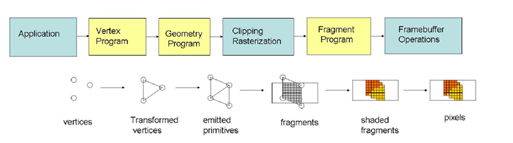
\includegraphics[width=5.34091in,height=1.48711in]{images/19_shader_pipeline.png}
	\caption{Wizualna reprezentacja kolejnych etapów rysowania przy pomocy shader'ów. \cite{researchgate:openglpipeline:2024}}
	\label{fig:shader_pipeline} % Dodano etykietę dla odniesień
\end{figure}

\subsection{Compute shader}
Konstrukcja współczesnych układów graficznych pozwala na ich
wykorzystanie poza dziedziną rysowania grafiki. Algorytmy korzystające z
szerokiej wielowątkowości i równoległości skorzystają także z
uruchamiania na GPU. Do tego celu stworzone zostały shader'y
przetwarzające (ang. \emph{\textbf{Compute Shader}}), wprowadzone przy
okazji Direct3D 11.

Programy takiego typu mogą, ale nie muszą być wykorzystywane jako pomoc
do generowania grafiki. Algorytmy kryptograficzne, rekonstrukcja skanów
tomogarfii komputerowej, przetwarzanie wideo, czy szczególnie dziś
powszechne uczenie maszynowe to tylko kilka przykładów wykorzystania
GPGPU (ang. \emph{\textbf{General Purpose Graphics Processing Unit}}) we
współczesnym świecie.

\subsection{Mesh shaders}
Ze względu na ewolucję sprzętową układów graficznych dotychczasowa
konstrukcja ścieżki rysowania przestała w optymalny sposób oddawać
niskopoziomowy sposób ich działania. Architektura SIMD (ang.
\emph{\textbf{Single Instruction Multiple Data}}) lepiej odpowiada
shader'om typu Compute, niż Vertex. Compute shaders mają niestety wadę w
postaci braku integracji z resztą pipeline'u renderowania, a co za tym
idzie konieczność zapisu i odczytu do pamięci głównej karty graficznej,
co wyraźnie spowalnia ich działanie. Z tego powodu Microsoft w DirectX 12 Ultimate wprowadził obsługę tzw.
\emph{\textbf{Mesh Shaders}}. Zastępują one pierwszą część ścieżki
rysowania, czyli Vertex, Geometry oraz Tesselation shaders i przekazują
swoje wyjście bezpośrednio do procesu rasteryzacji. Swoją konstrukcją
przypominają Compute shaders, lecz są zintegrowane bezpośrednio w
strumieniu danych rysowania klatki obrazu.

\section{Zaawansowane rozszerzenia Direct3D} % Zmieniono z enumerate

W czasie istnienia D3D układy graficzne i techniki rysowania obrazu
ewoluowały z prostego schematu \emph{Fixed Function Pipeline}, do
bardziej zaawansowanych, programowalnych shader'ów. Dodatkowe efekty
graficzne często wiązały się jednak z koniecznością dodatkowych
optymalizacji z uwzględnieniem sprzętowej akceleracji. Przedstawione
poniżej technologie są przykładami takich funkcji.

\subsection{WARP}
Skrót od \emph{\textbf{Windows Advanded Rasterization Platform}}. Jest
to programowy rasterizer pozwalający na uruchamianie aplikacji opartych
o Direct3D z użyciem rysowania programowego, bez akceleracji sprzętowej
układu graficznego. Wprowadzony w Windows 7 pierwotnie obsługiwał jedynie DirectX w wersji
10, współcześnie na systemie Windows 11 obsługuje pełny standard DirectX
12 Ultimate.

\subsection{Direct2D}
Interfejs programistyczny analogiczny do Direct3D, ale służący do
rysowania wektorowej grafiki dwuwymiarowej. Posiada wsparcie dla
rysowania przy pomocy CPU i GPU, krzywych Bezier'a, metod blending'u,
wypełniania i obrysowywania kolorem, a także rysowania sprite'ów. Najnowszym wydaniem jest Direct2D 1.3 wypuszczony wraz z Windows 10.

\subsection{DirectWrite}
Bardzo często wykorzystywaną funkcją, szczególnie w aplikacjach
użytkowych jest rysowanie tekstu. Funkcja taka przydaje się też często w
akcelerowanych sprzętowo silnikach rysujących interfejs aplikacji, bądź
jako nakładka interfejsu do gier. Proces renderowania wysokiej jakości i czytelności tekstu jest
skomplikowany. Z tego powodu powstało rozszerzenie DirectWrite, które
ułatwia ten proces. Z jego pomocą możliwe jest akcelerowane sprzętowo
rysowanie tekstu ze wsparciem Microsoft ClearType, czy OpenType. Do
działania wymagany jest system operacyjny Windows 7 lub wyżej.

\subsection{DirectX Ray-Tracing}
W skrócie \emph{\textbf{DXR}}. Wprowadzony w Direct3D 12 interfejs
akceleracji sprzętowej rozwiązań śledzenia promieni. Aplikacja uzupełnia
modelami nowo wprowadzoną strukturę drzewa, będącą akceleratorem
wykrywania kolizji promieni i wielokątów. Następnie przeprowadzane jest
śledzenie promieni, które przy odbiciach wywołuje nowe, specjalne
shader'y typu RT decydujące o sposobie odbicia i kolorze.

\subsection{DirectStorage}
Współczesne programy, a w szczególności gry potrzebują ogromnej ilości
zasobów wczytanych do pamięci układu graficznego. Proces ten jest
czasochłonny, ze względu na konieczność wczytania danych z nośnika,
dekodowania przez procesor centralny i wgrania na układ graficzny
najczęściej magistralą PCI-E. Firma Microsoft podjęła więc decyzję o stworzeniu API DirectStorage jako
część Direct3D 12. Pozwala ono na ominięcie CPU w procesie wczytywania i
odczyt danych bezpośrednio z nośnika typu SSD NVME do pamięci karty
graficznej. Obecnie nie jest to zbyt rozpowszechnione rozwiązanie, ale w
przyszłości może pozwolić na znaczące przyspieszenie wczytywania gier, a
nawet na zupełne wyeliminowanie ekranów ładowania.

\section{Alternatywne implementacje Direct3D na inne platformy.} % Zmieniono z enumerate

DirectX, a co za tym idzie Direct3D są interfejsami oficjalnie
wspieranymi jedynie na systemie Microsoft Windows. Jednak użytkownicy
innych systemów operacyjnych także chcieli mieć możliwość korzystania z
aplikacji napisanych w tym standardzie. Z tego powodu powstało kilka
implementacji standardu na systemy klasy Unix.

\subsection{DXVK}
Implementacja DirectX 8 do 11, będąca warstwą translacji między DirectX,
a Vulkan \cite{github:dxvk:2024}. Wspiera systemy Linux, a także możliwość uruchomienia
na systemie Windows. Posiada częściowe i nieoficjalne wsparcie dla
systemu Apple macOS. Jest częścią podsystemu Proton, będącego warstwą
kompatybilności opartą o moduł Wine pozwalającą uruchamiać gry i
aplikacje zgodne z API Windows na systemach Unix.

\subsection{VKD3D}
Moduł analogiczny do DXVK, ale pozwalający na uruchamianie aplikacji
zgodnych z DirectX 12. Posiada wsparcie dla systemów Linux i Windows. Najnowsze odsłony od wersji 2.11 posiadają wsparcie dla modułu DXR.